\chapter*{Introduction}
\addcontentsline{toc}{chapter}{Introduction}


\chapter{Document Classification}
    In this chapter we introduce a problem of document classification and commonly used approaches to this problem.
    
    \section{Machine learning}
        \subsection{Supervised machine learning}
        Supervised learning is a standard approach in machine learning. 
        Supervised algorithms learn to predict the best outputs for a given input.
        We denote the collection of input data, features, as $X$ and the corresponding expected outputs, labels, as $Y$.
        $X$ is usually a matrix of real values where rows of this matrix are individual samples.
        $Y$ is usually a vector of real values or integers. 
        We refer to the pair of features and labels $(X, Y)$ as a dataset.
        
        Learning is usually done by optimizing parameters $\Theta$ of a parametrized function $f_\Theta$,
        with regards to a loss function $E_y(\hat{y})$. 
        We refer to function $f_\theta$ as a \textit{model}.
        Common loss is an $L2$ loss function $$E_y(\hat{y}) = \frac{1}{2}(y - \hat{y})^2 = \frac{1}{2}\sum_{i=1}^n (y_i - \hat{y})^2$$.  
        Formally we want to find parameter $\hat{\Theta}$ such that $\hat{\Theta} = argmin_\Theta \left(E_y(f_\Theta(x) \right)$. 
        This equation is usually not solved directly, but through an optimization process called learning \cite{Goodfellow-et-al-2016}. % deep learning book
        
        \subsubsection{Gradient descent}

        \textit{Gradient descent} method finds local minima of a usually multivariate function. 
        This is a well suited approach to use in context of supervised machine learning. 
        
        We use an observation, that if we follow the opposite direction of the function in a given point, 
        we arrive in a local minima. Example is on the picture \* %\ref{obr:gradient}.
        
        In a context of machine learning, we optimize a cost function $Q$ of parameters $\Theta$, 
        $$Q(\Theta) = E_y(f_\Theta(x))$$. We follow the opposite direction of gradient of the cost function $Q$ in respect to parameters $\Theta$. We initialize $\Theta_0$ to small random numbers and we perform an gradient descent step
        
        $$\Theta^{t+1} = \Theta^t - \alpha \frac{\partial Q(\Theta^t)}{\partial \Theta^t} = \Theta^t - \alpha \nabla Q(\Theta^t)$$
        
        $\alpha$ denotes the size of the step we will make and is commonly known as a learning rate. 
        We perform the gradient descent step until we are not improving enough any more. 
        Formally we stop, when $|\Theta^{t+1} - \Theta^t| < \epsilon$ for a given $\epsilon$ \cite{bottou-bousquet-2008}.
        
        This process is also sometimes refered to as a batch gradient descent.

        \begin{figure}
        \centerline{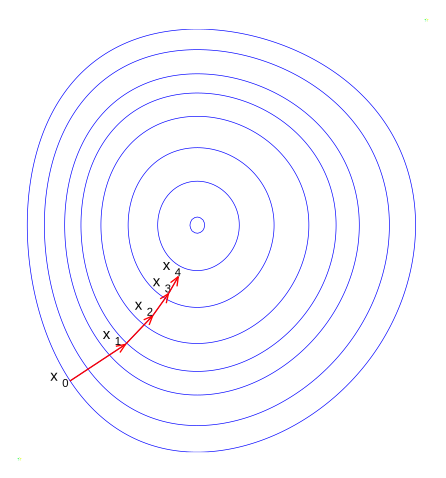
\includegraphics[width=0.4\textwidth]{images/gradient_descent}}
        \caption[Gradient descent]{Gradient descent \cite{pict} \*}
        \label{obr:gradient}
        \end{figure}
        
        
        \subsubsection{Stochastic gradient descent}
        
        During each gradient descent step, we need to go evaluate the gradient of the loss function over the whole dataset. 
        This is usually not feasible for larger datasets. 
        
        We can exploit the usual the cost function $Q$ can be rewritten as a sum of costs for each data point.
        
        $$Q(\Theta) = \sum_{i=1}^n Q_i(\Theta)$$
        
        $Q_i(\Theta)$ denotes the cost function computed on only the $i$-th element. 
        Finally we perform the gradient step for each example. 
        
        $$\Theta^{t+1} = \Theta^t - \alpha \frac{\partial Q_i(\Theta^t)}{\partial \Theta^t} = \Theta^t - \alpha \nabla Q_(\Theta^t)$$
        
        \* 
        For apropriate $\alpha$ we usually see a much faster convergence than for gradient descent.
        
        
        \subsection{Feed forward neural network}
        There is a lot of ways how to construct function $f_\theta$ that we want to optimize. 
        One of the most popular ones is roughly inspired by the human brain and is called a \textit{feed forward neural network}.
        
        Neural network consists of small interconnected computational units (neurons) that are usually organized into a layers.
        Each unit takes some inputs, based on them produces an output and sends it to other units. 
        In a feed forward neural network, the signal is always moving forward,
        hence unit on the $k$-th layer can only take it's input from previous layers \cite{Goodfellow-et-al-2016}.
        
        By adjusting the connections and theirs strengths, the network can learn to produce a specific output for a specific input.
        
        Simple neural network can be seen on an image \ref{obr:siet}.
        
        \begin{figure}
        \centerline{\includegraphics[width=0.4\textwidth]{images/siet}}
        \caption[Simple neural network with 2 layers, 3 inputs, 4 neurons and 2 outputs]{Simple neural network with 2 layers, 3 inputs, 4 neurons and 2 outputs\*} % redraw
        \label{obr:siet}
        \end{figure}
        
        The simplest model for a unit is weighted sum and application of some function. 
        Formally the unit receives a vector of inputs $x$ and computes output $g(\sum_{i=1}^n w_i x_i)$, 
        where $w_i$ is a connection strength to the $i$-th input.
        This one unit can be viewed as a simple one layer neural network with one output.
        
        Common realizations of function $g$ are: logistic function $g(x) = \frac{1}{1+e^{-x}}$, 
        hyperbolic tangent $g(x)=\frac{e^x-e^{-x}}{e^x+e^{-x}}$, relu $g(x) = \max(0,x)$ or leaky relu $g(x)=\log(1+\exp(x))$
        
        One layer of such units can be compactly described thanks to matrix notation as
        $$y=g(X W)$$
        
        $X$ represents the input matrix (number of samples $n$ times number of features $k$) and $W$ is the matrix of weights (number of features $k$ times number of units $u$). Note that function $g$ is applied element-wise.
        
        The important observation is, that we can chain such layers to from deeper neural networks.
        $$y=g(g(X W_1) W_2)$$
        
        $W_1$ are weight of hidden neurons and $W_2$ are weight of output neurons.
        There is no consensus in the community about how to count the layers. 
        For example the simple network on picture \ref{obr:siet} could be seen as a $3$ layer neural network,
        because it has input units, hidden units and output units.
        In this thesis we will use the number of matrices $W$ that crates the model.
        
        This family of functions is very broad and can in fact approximate any function \cite{cybenko1989approximation}.
        However, we need to train them first.
        
        \subsubsection{Back propagation}
        
        Back propagation is a method for effective computation of the gradient of a neural network.
        It relies on the the fact, that neural networks are just a simple compositions of matrix multiplications 
        and function applications. 
        It also relies on the fact, that functions used in the units are differentiable (almost everywhere).
        
        Backpropagation works in two parts, forward pass and backward pass.
        In the forward pass we feed to input to the network, compute acctivations of each layer and compute the final output.
        In the seccont pass, we make use of the chain rule and incrementally compute gradient with respect to each layer of the network.
        Then we use the gradient descent and optimize the parameters \cite{rumelhart1986david}.
        
        \* %example
        %Let's take for example the simple 2 layer neural network $y=g(g(X W_1) W_2)$ with the $L2$ loss. 
        %Let $h_1=g(X W_1)$. 
        %We need to compute $\frac{\partial Q(W_2)}{W_2} = \frac{E_y(g(h_1 W_2))}{\partial W_2}$. 
        %By using the chain rule we get 
        %$\frac{E_y(g(h_1 W_2))}{\partial W_2} = 
        %\frac{\partial E_y(\hat{y})}{\partial \hat{y}}\frac{\partial \hat{y}}{\partial W_2}$
        
        
        
        
        
    \section{Word vectors}
        \subsection{distributed vs local representation, count based, prediction based}
        \cite{Rubenstein:1965:CCS:365628.365657} % distributional hyphotesis. 
        \cite{maas2011learning} % lda, vector space model

    \section{Prediction based word vectors}
        \subsection{Word vectors}
        \cite{DBLP:journals/corr/MikolovSCCD13} % podvzorkovanie.
        \cite{DBLP:conf/icml/LeM14} % slovne vektory
        \cite{rong2014word2vec} % some word2vec shit
        \cite{pennington2014glove} % glove word vectors




    \section{Count based word vectors}
        \cite{wiemer2004latent} % Latent semantic analysis
        Latent Dirichlet allocation
        Explicit semantic analysis
        Latent semantic analysis
        Hierarchical Dirichlet process
        Non-negative matrix factorization
        \subsection{SVD}
        {$$
\begin{matrix} 
 M &  ~~ U & \Sigma & V^T \\
 \textbf{t}_j^T &  & &  \\
 \downarrow &  & &  \\
(\textbf{d}_i) \rightarrow 
\begin{bmatrix}
x_{1,1} \dots  x_{1,n} \\
\vdots ~~~  \ddots ~~~ \vdots \\
x_{i,1} \dots  x_{i,n} \\
\vdots ~~~ \ddots ~~~ \vdots \\
x_{m,1} \dots  x_{m,n} \\
\end{bmatrix}
=
&
\textbf{u}_i \rightarrow
\begin{bmatrix} 
\begin{bmatrix} & \textbf{u}_1 & \end{bmatrix} \\
\vdots \\
\begin{bmatrix} & \textbf{u}_l & \end{bmatrix}
\end{bmatrix}
&
\cdot
\begin{bmatrix} 
\sigma_1 \dots ~~~ 0 \\
\vdots ~~~ \ddots  \vdots \\
0  \dots  \sigma_l \\
\end{bmatrix}
&
\cdot
\begin{bmatrix} 
\begin{bmatrix} \, \\ \, \\ \textbf{v}_1 \\ \, \\ \,\end{bmatrix} 
\dots
\begin{bmatrix} \, \\ \, \\ \textbf{v}_l \\ \, \\ \, \end{bmatrix}
\end{bmatrix}
\end{matrix}
$$}
        \subsection{Truncated SVD}
        \subsection{Iterated SVD}
            \cite{brand2006fast} % incremental svd
        \subsection{Relationship to Word2Vec}
            \cite{naili2017comparative} % wrf is this? some comparison
            \cite{levy2014neural} % word2vec as matrix factorization
            \cite{altszyler2016comparative} % lsa vs word2vec on samall corpora
            \cite{levy2015improving} % word2vec hacks in lsi


    \section{Weight schemes}
        \cite{wu2017balancing} % word weights
            weight schemes
            Supervised weight scheme



\chapter{Related work}
    \section{Class knowledge into LSI}
        \subsection{Supervised LSI}
            \cite{sun2004supervised} %supervised lsi, discriminative basis

        \subsection{Sprinkling}
            \cite{chakraborti2007supervised} % Sprinkling
        
        \subsection{Supervised weights}
            \cite{ji2013discriminative} % TF KLD
            \cite{deng2014study} % supervised weights
            \cite{lan2009supervised} % supervised weights for text categorization

    
    \section{SVD in neural networks}
        \subsection{SVD as structured layer} 
            \cite{ionescu2015training} % svd in neural networks

    
\chapter{Model design}
    \section{Goals and motivation}
    \section{Design}
    \section{Implementation}
        \subsection{gensim lsa}
        \subsection{tensorflow for clasifier?}
    \*
\chapter{Experiments and evaluation}

    Performance
    
    Result analysis
    
    Weight analysis
    
    Transfer learning?

    \section{Classification datasets}
        \subsection{all datasets}
            \cite{conneau2017supervised} % datasets, benchmarks

    \section{Interpretability}
        \cite{ribeiro2016should} % explainability


